\documentclass[12pt,a4paper]{article}

\usepackage[T1]{fontenc}
\usepackage{amsmath, amssymb, amsfonts}
\usepackage[magyar]{babel}
\usepackage[utf8]{inputenc}
\usepackage{graphicx}
\usepackage{graphics}
\usepackage{mathtools}
\usepackage{epsfig}
\usepackage{epstopdf}
\usepackage{cite}
\usepackage{caption}
\usepackage{hyperref}
\usepackage[bottom=4cm]{geometry}
%\geometry{a4paper, portrait, margin=1in}

\title{\huge{Korszerű vizsgálati módszerek labor jegyzőkönyv}\\ \vspace{20pt}
\textbf{Röntgendiffrakció}}

\author{\Large{\textsc{Csörnyei Géza}} \vspace{10pt}\\
	\textrm{Eötvös Loránd Tudományegyetem}\\
	\textrm{Fizika BSc III. évfolyam}
	}
\date{}
%\lhead{}
\begin{document}
\addtolength{\voffset}{-1.0cm}
\addtolength{\textheight}{1.0cm}
\begin{titlepage}
\maketitle

\begin{figure}[!htb]
\centering

\includegraphics[scale=0.6]{eltecimer.jpg}
\end{figure}

\hfil \Large{'C' mérőcsoport}\hfil  \\
\vspace*{2pt}
\hfil \Large{\emph{Mérés dátuma:} 2018.04.12.}\hfil \\
\vspace*{2pt}
\hfil \hspace*{45pt} \Large{\emph{Mérés vezetője:} Heczel Anita}\hfil
\thispagestyle{empty}
\end{titlepage}

\section{Bevezető}
\hspace*{10pt} A laborgyakorlat során a röntgendiffrakciós mérés menetével, valamint az ahhoz használt eszközökkel ismerkedhettünk meg. A gyakorlat során a pordiffrakciós mérések alapján meghatároztuk a FeAl rácstípusát a reflexiók indexelésének segítségével,  majd meghatároztuk egy mechanikai ötvözéssel előállított Al(Mg) ötvözet Mg tartalmát, meghatároztunk egy ismeretlen fázist és annak szemcseméretét, valamint meghatároztuk egy adott Si minta pordiffrakciós méréséből annak rácsparaméterét.

\section{Mérés kiértékelése}
\subsection{Rácstípus meghatározása}
\hspace*{10pt} A laborgyakorlat során az első feladatunk egy már korábbról rendelkezésre álló, FeAl minta pordiffrakciós méréséből történő rácstípus meghatározás volt. A rácstípus meghatározását a reflexiók indexelésével tudjuk elvégezni, mely az \ref{fig:1} . ábrán látható.\\
\begin{figure}[!h]
\centering
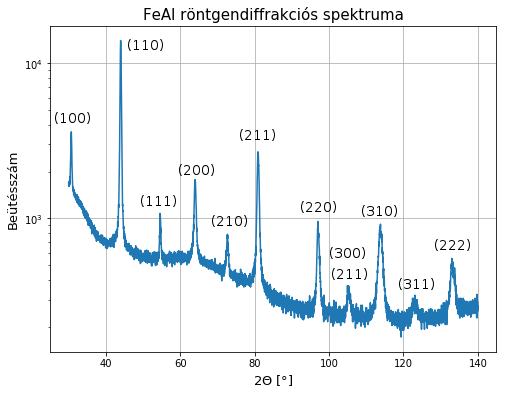
\includegraphics[scale=0.75]{FeAl_ind}
\caption{A beütésszám a szóródási szög kétszeresének függvényében a FeAl minta esetén}
\label{fig:1}
\end{figure}
\newpage
A diffraktogramról csúcsok helyeit leolvasva ki tudjuk számolni a z azokhoz tartozó rácssíktávolságokat a Bragg-egyenlet segítségével, amely
$$ 2d_{hkl} \cdot \sin \Theta = \lambda ,$$
ahol $d_{hkl}$ a $\{hkl\}$ indexekkel jellemzett síksereghez tartozó rácssíktávolság, $\lambda$ a röntgenfotonok hullámhossza, $\Theta$ pedig a szóródás szöge. A hullámhossz itt a réz $K\alpha$ vonalainak súlyozott hullámhossza, 0.15418 nm volt. A mérés során feltételeztük, hogy egy köbös kristályrácsról van szó, azonban ezen belül a típusát nem ismertük. Köbös kristályrács esetén a következő összefüggés igaz a rácssíktávolságokra:
$$\frac{1}{d_{hkl}^2}=\frac{1}{a^2}(h^2+k^2+l^2)=\frac{N}{a^2},$$
ahol $a$ a rács rácsállandója. A diffraktogramról leolvasható szögek segítségével ki tudjuk számolni, mely $N$ értékek esetére jelennek meg diffrakciós csúcsok, és ez alapján pedig különböző táblázatok segítségével ki tudjuk keresni, milyen az adott anyag rácsszerkezete. A rácssíktávolságok számolása és az indexeknek történő megfeleltettetése után az alábbi táblázatot kaptuk (\ref{tab:1}):\\
\begin{table}[!h]
\begin{center}
\begin{tabular}{|c|c|c|c|}
\hline
$ 2\Theta [^{\circ}]$ &  $d_{hkl} $ [nm] & $\frac{1}{d_{hkl}^2}$ [$\frac{1}{\textrm{nm}^2}$] & $N$ \\
\hline
30.68 & 0.291 & 11.776 & 1 \\
\hline
43.97 & 0.206 & 23.583 & 2 \\
\hline
54.68 & 0.168 & 35.493 & 3 \\
\hline
63.97 & 0.146 & 47.213 & 4 \\
\hline
72.67 & 0.130 & 59.073 & 5 \\
\hline
81.02 & 0.119 & 70.973 & 6 \\
\hline
97.12 & 0.103 & 94.563 & 8 \\
\hline
105.31 & 0.097 & 106.349 & 9 \\
\hline
113.87 & 0.092 & 118.181 & 10 \\
\hline
123.10 & 0.087 & 130.080 & 11 \\
\hline
133.20 & 0.084 & 141.728 & 12 \\
\hline
\end{tabular}
\caption{A rácstípus meghatározásához leolvasott Bragg-szögek és a számolt rácsparaméterek, azok reciprok négyzetei, valamint a laborban kapott táblázat alapján az egyes szögekhez rendelt $N$ értékek.}
\label{tab:1}
\end{center}
\end{table}
\newline
A kapott értékekből látszik, hogy csak az $N=7$ eset nem látszott a felvételen (természetesen ez egyik köbösben sincs benne, mert nem áll elő három négyzetszám összegeként), viszont rajta kívül az összes többi jelen volt. Ez alapján kijelenthető, hogy a FeAl rácsszerkezete egyszerű köbös.
\newpage
\subsection{Ötvözőkoncentráció meghatározása}
\hspace*{10pt} Ezen feladat során egy mechanikai ötvözéssel előállított Al(Mg) ötvözet Mg tartalmát kellett meghatároznunk. A számítási folyamat eleje megegyezett az első feladatéval: egy diffraktogramról leolvastuk a Bragg-szögeket, majd kiszámítottuk ezekhez a rácssík távolságokat. A mérés során ismertnek tekinthettük az egyes csúcsokhoz tartozó indexeket, így minden $d_{hkl}$ esetére az ismert $N$-ekkel ki tudtuk számolni a megfelelő $a_{hkl}$ rácsparaméter értékeket. A rácsparaméter értékek és a hozzájuk tartozó Bragg-szögek között az alábbi kapcsolat áll fenn (Nelson-Riley formula):
$$a_{hkl}= a_0 - D \cdot \cos \Theta \cdot \left( \textrm{ctg}\Theta + \frac{\cos \Theta}{\Theta} \right)$$
Az ötvözőkoncentráció meghatározásához számunkra az $a_0$ érték a fontos, ugyanis ebből egy a laborban kapott kalibrációs egyenes segítségével ki tudjuk majd számolni a Mg atomszázalékát a mintában. A minta diffraktogramja a \ref{fig:2} . ábrán látható. 
\begin{figure}[!h]
\centering
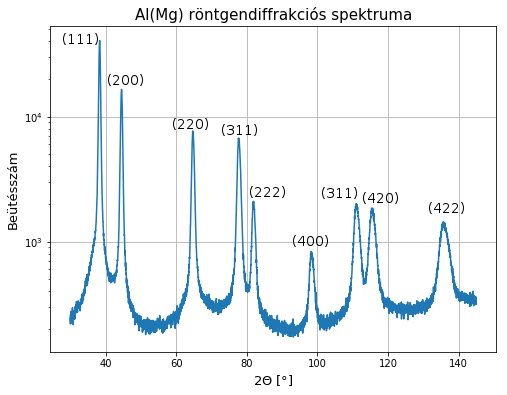
\includegraphics[scale=0.75]{AlMg_ind}
\caption{A beütésszám a szóródási szög kétszeresének függvényében a Al(Mg) minta esetén}
\label{fig:2}
\end{figure}
\newpage
A leolvasott és számolt értékeket a \ref{tab:2} . táblázat tartalmazza. Az egyszerűség érdekében a táblázatban bevezettük az
$$F(\Theta)=\cos \Theta \cdot \left( \textrm{ctg}\Theta + \frac{\cos \Theta}{\Theta} \right)$$
jelölést. \\
\begin{table}[!h]
\begin{center}
\begin{tabular}{|c|c|c|c|c|}
\hline
N & $2\Theta [^{\circ}]$ & $F(\Theta)$ & $d_{hkl}$ [nm] & $a_{hkl}$ [nm]  \\
\hline
3 & 38.37 & 5.379 & 0.2346 & 0.4063\\
\hline
4 & 44.48 & 4.471 & 0.2037 & 0.4074\\
\hline
8 & 64.83 & 2.589 & 0.1438 & 0.4068\\
\hline
11 & 77.81 & 1.8563 & 0.1228 & 0.4071\\
\hline
12 & 82.01 & 1.6636 & 0.1175 & 0.4070\\
\hline
16 & 98.50 & 1.0582 & 0.1018 & 0.4070\\
\hline
19 & 111.10 & 0.7181 & 0.0935 & 0.4075\\
\hline
20 & 115.83 & 0.6121 & 0.0910 & 0.4069\\
\hline
24 & 135.96 & 0.2701 & 0.0832 & 0.4074\\
\hline
\end{tabular}
\caption{Az ötvözőkoncentráció meghatározásához szükséges mennyiségek táblázata}
\label{tab:2}
\end{center}
\end{table}
\newline
Amennyiben a táblázatban szereplő $a_{hkl}$ és $F(\Theta)$ adatokra egyenest illesztünk, akkor fentiek értelmében meg tudjuk határozni az $a_0$ rácsparamétert. Az egyenesillesztés a \ref{fig:3} . ábrán látható.\\
\hspace*{10pt} Az illesztett egyenes egyenletéből megkapható a rácsparaméter értéke, amely 
$$ a_0 = (0.407269 \pm 1.713 \cdot 10^{-4}) \hspace*{5pt} \textrm{nm} .$$ Ezen érték és a \ref{fig:4} . ábrán látható kalibrációs egyenes egyenletével meghatározhatjuk az ötvözetben levő ötvözőanyag atomszázalékát.
\newpage
\begin{figure}[!h]
\hspace*{-0.5cm}
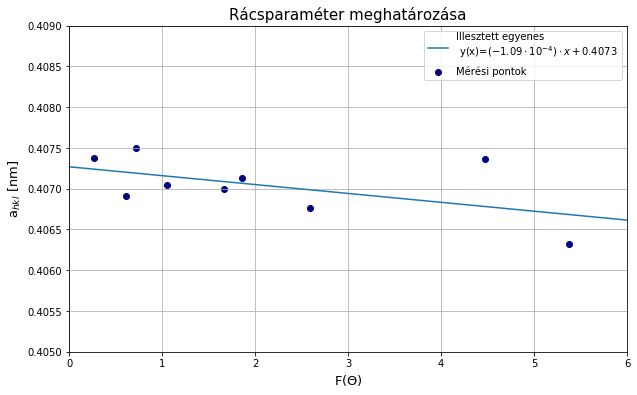
\includegraphics[scale=0.65]{otvoz}
\caption{A rácsparaméter meghatározásához készített egyenesillesztés}
\label{fig:3}
\end{figure}
\begin{figure}[!h]
\centering
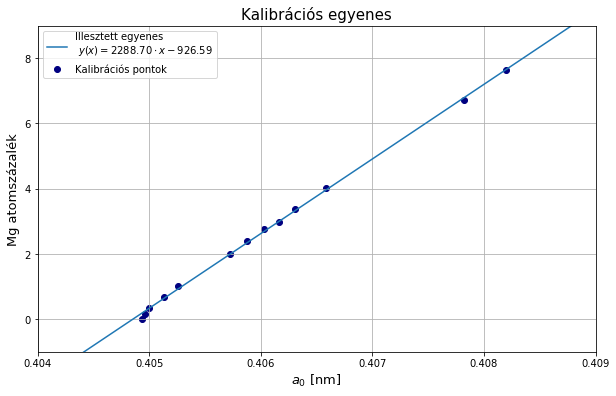
\includegraphics[scale=0.65]{kalib}
\caption{Az ötvözőanyag atomszázalék és a rácsparaméter közötti arányosság. A kalibrációnak nyilvánvalóan nincs értelme negatív atomszázalék értékekre, csupán a jobb láthatóság miatt ábrázoltam azon tartományon is}
\label{fig:4}
\end{figure}
\newpage
A kalibrációs egyenes egyenlete:
$$y(x)= (2288.701 \pm 22.120) \cdot x - (926.592 \pm 8.981).$$
Ha ezen egyenletbe behelyettesítjük az általunk kapott rácsparamétert, akkor megkapjuk a keresett atomszázalékot. A behelyettesítés után kapott érték:
$$M_{at}=(5.525 \pm 0.076) \% ,$$
ahol a hibát az illesztésekből származó relatív hibák terjedésével számoltam az alábbi képlet szerint, amelyben $m$ és $b$ a kalibrációs egyenes meredeksége és tengelymetszete:
$$\Delta M_{at} = M_{at}\sqrt{\left(\frac{\Delta a_0}{a_0} \right)^2 + \left(\frac{\Delta m}{m}\right)^2 + \left(\frac{\Delta b}{b}\right)^2}.$$
Mivel ismertek az alumínium és a magnézium moláris tömegei ($M_{Al}$=26.98 $\frac{\mathrm{g}}{\mathrm{mol}}$ és $M_{Mg}$=24.31 $\frac{\mathrm{g}}{\mathrm{mol}}$), ezért ezt az atomi százalékot át tudjuk váltani súlyszázalékra is, az alábbi képlet segítségével:
$$M_{s}=\frac{M_{at} \cdot M_{Mg}}{M_{at}\cdot M_{Mg} + (100-  M_{at})\cdot M_{Al}}.$$
Ez alapján az ötvözőanyag súlyszázaléka az ötvözetben
$$M_s=(5.006 \pm 0.069) \% ,$$
ahol a hibát a relatív hiba terjedésével, jelen esetben megmaradásával számoltam. 
\newpage
\subsection{Ismeretlen fázis azonosítása}
\hspace*{10pt} Ebben a feladatban a laborban rendelkezésünkre álló adatbázisok (ICDD) segítségével azonosítanunk kellett egy ismeretlen fázist a mért diffraktogram alapján. A kapott diffraktogram a \ref{fig:5} . ábrán látható.\\
\begin{figure}[!h]
\centering
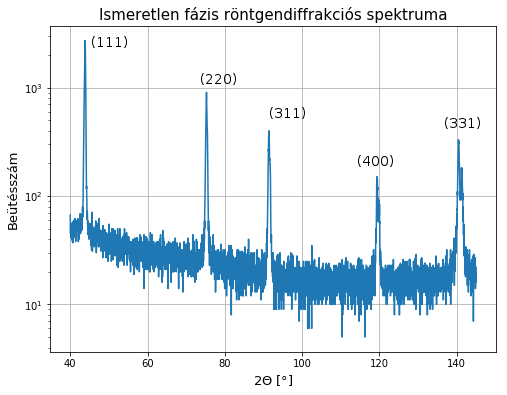
\includegraphics[scale=0.75]{ism_ind}
\caption{A beütésszám a szóródási szög kétszeresének függvényében a ismeretlen minta esetén}
\label{fig:5}
\end{figure}
\newline
A fent már többször is használt módon kiszámoltuk az rácssík távolságokat az egyes reflexiós csúcsok esetére. Az adatbázisban történő kereséshez a három legnagyobb intenzitású csúcsot használtuk, de szükség esetén a több csúcsot is hozzávehettünk volna, ha kevesebb esetén lett volna még átfedés az egyes anyagok között. A számolt értékek a \ref{tab:3} . táblázatban vannak felsorolva.
\begin{table}[!h]
\begin{center}
\begin{tabular}{|c|c|}
\hline
2$\Theta$ $[^{\circ}]$ & $d_{hkl}$ [nm] \\
\hline
43.81 & 0.2065 \\
\hline
75.29 & 0.1262 \\
\hline
91.44 & 0.1076 \\
\hline
119.41 & 0.0892 \\
\hline
140.68 & 0.0818 \\
\hline
\end{tabular}
\caption{Ismeretlen anyaghoz számolt rácssíktávolságok}
\label{tab:3}
\end{center}
\end{table}
\newline
Az adatbázisban található adatokkal történő összevetésből azt az eredményt kaptuk, hogy az ismeretlen anyag gyémánt volt.\\
\hspace*{10pt} A vizsgált anyag beazonosítása után a krisztallitméret meghatározását kaptuk feladatul, melyhez a diffraktogramon látható első csúcsot vettük alapul. A csúcsok azon tulajdonsága, melyből a szemcseméretre következtetni lehet, a kiszélesedésük. Ennek két fő okozója van: az egyik instrumentális eredetű, a másik a szemcsemérettől függ. Alapesetben fellépne a rácshibák miatti vonalkiszélesedés hatása is, azonban ez a Bragg-szöggel arányosan nő (míg a szemcseméret hatása azzal fordítottan arányos), így amennyiben a legkisebb szöghöz tartozó csúcsot tekintjük, akkor a rácshibák okozta kiszélesedés elhanyagolható lesz a másik kettő mellett. Ezáltal a szemcsemérethez köthető vonalkiszélesedés az alábbi alakban adható meg:
$$\beta_f = \sqrt{\beta^2 -\beta_i ^2} ,$$
ahol $\beta$ az integrális vonalkiszélesedés, melyet a labor számítógépére telepített $Origin$ nevű programmal határoztunk meg, valamint $\beta_i$ az instrumentális vonalkiszélesedés, amely megegyezne az integrális vonalkiszélesedéssel egy kellően kis szemcsékből álló, nagy méretű, közel hibátlan kristály esetén. A kapott mérés esetében $\beta_i=0.1^{\circ}$ és $\beta=(0.27019 \pm 0.020) ^{\circ}$ voltak, ahol a hiba a szögfelbontás és a program pontossága alapján volt becsülhető. Ebből a szemcseméret következtében keletkezett vonalkiszélesedés paramétere:
$$\beta_f=(0.251 \pm 0.018)^{\circ}=(4.381 \pm 0.324)\cdot 10^{-3}\hspace*{5pt} \mathrm{rad}.$$
A térfogattal súlyozott szemcseméret az [1]-ben olvasottak alapján a következő képletből származtatható:
$$<x>_{vol}=\frac{4\lambda}{3\beta_f \cos\Theta}.$$
Ebben az esetben a számítás hibáját az alábbi formula adja a relatív hibák terjedésének megfelelően:
$$\Delta <x>_{vol}=<x>_{vol} \sqrt{\left(\sin\Theta   \frac{\Delta \Theta}{\Theta} \right)^2+\left(\frac{\Delta \beta_f}{\beta_f}\right)^2}.$$
Ez alapján a számolt szemcseméret:
$$<x>_{vol} = (50.591 \pm  3.628)\hspace*{5pt} \mathrm{nm} .$$
\newpage
\subsection{A TA minta rácsparaméterének meghatározása}
\hspace*{10pt} Az előzőekhez hasonló módon, ezen minta esetében is a diffraktogram kiértékelésével és a rácssíktávolságok kiszámolásával kezdtem a számításaimat. A mintához tartozó diffraktogram a \ref{fig:6} . ábrán látható.\\
\begin{figure}[!h]
\centering
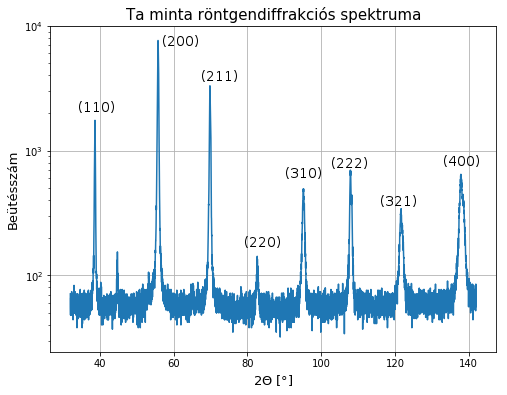
\includegraphics[scale=0.75]{ta_ind}
\caption{A beütésszám a szóródási szög kétszeresének függvényében a Ta minta esetén}
\label{fig:6}
\end{figure}
\newline
A számított értékeket a mintához kapott ICDD adatlapról leolvasott adatokkal kiegészítve az alábbi táblázat tartalmazza.
\begin{table}[!h]
\begin{center}
\begin{tabular}{|c|c|c|c|c|}
\hline
N & $2\Theta [^{\circ}]$ & $F(\Theta)$ & $d_{hkl}$ [nm] & $a_{hkl}$ [nm]  \\
\hline
2 & 38.67 & 5.378 & 0.2346 & 0.3318 \\
\hline
4 & 55.80 & 3.273 & 0.1647 & 0.3295 \\
\hline
6 & 69.84 & 2.278 & 0.1347 & 0.3298 \\
\hline
8 & 82.56 & 1.640 & 0.1168 & 0.3305 \\
\hline
10 & 95.17 & 1.164 & 0.1044 & 0.3302 \\
\hline
12 & 107.94 & 0.795 & 0.0953 & 0.3302 \\
\hline
14 & 121.59 & 0.4971 & 0.0883 & 0.3304 \\
\hline
16 & 137.87 & 0.2458 & 0.0826 & 0.3304 \\
\hline
\end{tabular}
\end{center}
\end{table}
\newpage
A rácsparaméter számítását itt is a Nelson-Riley törvény segítségével végeztem. A már korábban bemutatott összefüggés alapján egyenest illesztettem a számolt adatokra, melyet a \ref{fig:7} . ábrán ábrázoltam. \\
\begin{figure}[!h]
\hspace*{-0.5cm}
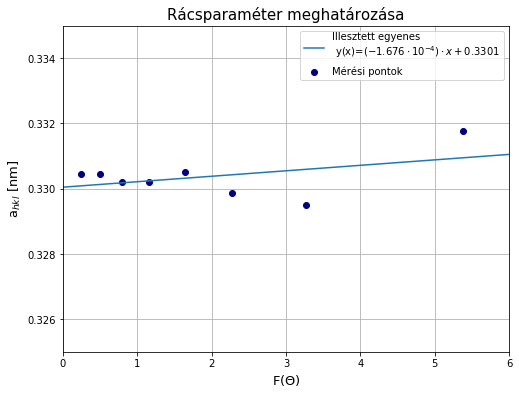
\includegraphics[scale=0.75]{ta}
\caption{A rácsparaméter meghatározásához készített egyenesillesztés}
\label{fig:7}
\end{figure}
\newline
Az illesztett egyenes egyenlete
$$ a_{hkl} = (0.33005 \pm 0.0003) \hspace*{5pt} \mathrm{nm} \hspace*{5pt} + (1.6760 \pm 1.4020)\cdot 10^{-4} \hspace*{5pt} \mathrm{nm} \cdot F(\Theta),$$
amelyből tehát a keresett rácsparaméter értéke 
$$a_0=(0.33005 \pm 0.0003) \hspace*{5pt} \mathrm{nm},$$
ami közelítőleg megegyezik a kapott adatlapon olvasható $a_{0,\textrm{adatlap}}=0.33058$ nm értékkel.
\newpage
\section{Diszkusszió}
\hspace*{10pt} Mérésünk során betekintést nyertünk a röntgendiffrakció mérésének módszertanába, valamint több ezen módszerrel végzett mérést is kiértékeltünk és az általunk kapott eredmények a mérés és kiértékelés pontosságán belül megegyeznek a korábbi mérésekből származó, az ICDD adatlapokon megtalálható értékekkel. Megjegyzendő, hogy a kiértékelés hibáját főként a csúcsok helyzetének közelítő meghatározása volt, amennyiben ezen pozíciómeghatározást nem leolvasással, hanem csúcsot és a hátteret leíró valamilyen függvény illesztésével végeznénk, úgy a kapott eredmények pontosabbak lehetnének.

\section*{Hivatkozások}
\hspace*{14pt} [1] : \emph{Méréshez kiadott jegyzet}:\\
\hspace*{34pt} \texttt{http://atomfizika.elte.hu/kvml/docs/korszeruosszefuzott.pdf}\\
\end{document}